\documentclass[12pt]{article}

\usepackage{tabularx}
\usepackage{booktabs}
\usepackage{fullpage}
\usepackage{graphicx}

%% Comments

\usepackage{color}

\newif\ifcomments\commentstrue %displays comments
%\newif\ifcomments\commentsfalse %so that comments do not display

\ifcomments
\newcommand{\authornote}[3]{\textcolor{#1}{[#3 ---#2]}}
\newcommand{\todo}[1]{\textcolor{red}{[TODO: #1]}}
\else
\newcommand{\authornote}[3]{}
\newcommand{\todo}[1]{}
\fi

\newcommand{\wss}[1]{\authornote{blue}{SS}{#1}} 
\newcommand{\plt}[1]{\authornote{magenta}{TPLT}{#1}} %For explanation of the template
\newcommand{\an}[1]{\authornote{cyan}{Author}{#1}}

%% Common Parts

\newcommand{\progname}{Flick Picker}
\newcommand{\authname}{Team 7, 7eam
\\ Talha Asif - asift
\\ Jarrod Colwell - colwellj
\\ Madhi Nagarajan - nagarajm
\\ Andrew Carvalino - carvalia    
\\ Ali Tabar - sahraeia
}     

\usepackage{hyperref}
    \hypersetup{colorlinks=true, linkcolor=blue, citecolor=blue, filecolor=blue,
                urlcolor=blue, unicode=false}
    \urlstyle{same}
                                


\begin{document}

\title{Software Requirements Specification for \progname: Group Show Finder} 
\author{\authname}
\date{\today}
	
\maketitle
\vspace*{\fill}
Created From: Volere, Requirements Specification Template, Edition 18


~\newpage \pagenumbering{roman}

\tableofcontents

~\newpage

\section*{Revision History}

\begin{tabularx}{\textwidth}{p{3cm}p{2cm}X}
\toprule {\bf Date} & {\bf Version} & {\bf Notes}\\
\midrule
Oct 1/22 & 0.0 & Copying Volere Template and updating sections\\
Oct 1/22 & 0.1 & Adding Sections 1, 3, 5\\
Oct 2/22 & 0.2 & Adding Section 6\\
\bottomrule
\end{tabularx}

~\newpage \pagenumbering{arabic}

\section{The Purpose of the Project}

\subsection{The User Business or Background of the Project Effort}
The business aims to make finding shows across groups of friends with differing preferences easier by streamlining the process from start to finish. As a quick summary, users will be able to input their preferences, make groups with their friends, and the group will get recommendations based on all their preferences. In addition, an opportunity arose in the market after COVID passed as large groups can create host gatherings for any events, one such that this application can select.

\subsection{Goals of the Project}
Goals can shift as development continues, entirely losing scope on the developers' passion for why the application started. Thus there will only be a few immediate goals to capture the passion that developers currently have and will continue to uphold in the future:
\begin{itemize}
	\item Provide a means of choosing a Movie, TV show, or Anime to watch immediately in a large friend group, which they all enjoy
	\item Users can be recommended a Movie, TV show, or Anime individually as well.
	\item Minimize the number of advertisements while using the application
\end{itemize}

\section{The Stakeholders}
a

\subsection{The Client}
a

\subsection{The Customer}
a

\subsection{Other Stakeholders}
a

\subsection{The Hands-On Users of the Product}
a

\subsection{Personas}
a

\subsection{Priorities Assigned to Users}
a

\subsection{User Participation}
a

\subsection{Maintenance Users and Service Technicians}
a

\section{Constraints}

\subsection{Solution Constraints}
There are no specific constraints the stakeholders have asked to be on the product regarding the solution. So instead, 7eam deems it necessary to have a general form of constraint on the development of Flick Picker that is the following:
\begin{itemize}
	\item Flick Picker must have in-depth tests on any part of the application before releasing it to the users and also follow a strict and healthy software engineering process
\end{itemize}
There are no specific technological constraints. However, the technology stack must follow industry standards.

\subsection{Implementation Environment of the Current System}
The application will be deployed on a website, so the restrictions of a browser follow.

\subsection{Partner or Collaborative Applications}
N/A

\subsection{Off-the-Shelf Software}
The list of Movies, TV Shows, and Anime will be polled from two separate APIs, which is the following:
\begin{itemize}
	\item MyAnimeList for data on Anime
	\item OMDB for data on TV Shows and Movies
\end{itemize}

\subsection{Anticipated Workplace Environment}
As Flick Picker is a browser application, 7eam expects users to use the application on their desktops or phones. Thus the application must be optimized for both possible settings, relying on a responsive layout. However, the users' physical workplace has no bearing on the design, as they can use it whenever necessary. 

\subsection{Schedule Constraints}
The schedule is the same as the one Dr. Smith has provided us with

\begin{tabular}{ |p{9.7cm} l|}
	\hline
	Team Formed, Project Selected & September 19\\
	\hline
	Problem Statement, Development Plan & September 26\\
	\hline
	Requirements Document Revision 0 & October 5\\
	\hline
	Hazard Analysis 0 & October 19\\
	\hline
	V\&V Plan Revision 0 & November 2\\
	\hline
	Proof of Concept Demonstration & November 14--25\\
	\hline
	Design Document Revision 0 & January 18\\
	\hline
	Revision 0 Demonstration & February 6--February 17\\
	\hline
	V\&V Report Revision 0 & March 8\\
	\hline
	Final Demonstration (Revision 1) & March 20--March 31\\
	\hline
	EXPO Demonstration & April TBD\\
	\hline
	Final Documentation (Revision 1)\newline 
	- Problem Statement\newline
	- Development Plan\newline
	- Requirements Document\newline
	- Hazard Analysis\newline
	- Design Document\newline
	- V\&V Plan\newline
	- V\&V Report\newline
	- User's Guide\newline
	- Source Code\newline & April 5\\
	\hline
\end{tabular}

\subsection{Budget Constraints}
The expenses for this application must not exceed \$500, and there are only five developers working on 7eam.

\subsection{Enterprise Constraints}
N/A

\section{Naming Conventions and Terminology}
a

\subsection{Glossary of All Terms, Including Acronyms, Used by Stakeholders Involved in the Project}
a

\section{Relevant Facts and Assumptions}

\subsection{Relevant Facts}
There is no existing solution 7eam has found that fills a similar role as selecting a Movie, TV Show or Anime based on the preferences of a group of users.


\subsection{Business Rules}
N/A

\subsection{Assumptions}
There are a few assumptions 7eam deems necessary to see regarding Flick Picker's capabilities and what it will not do:
\begin{itemize}
	\item Flick Picker will not provide a means to watch the selected show directly through the application
	\item Flick Picker will suggest the best movie, tv show, or anime for the group. This may violate the preferences of a member or multiple members of the group.
	\item The browser on which the application is used, through any device, is not deprecated
\end{itemize}

\section{The Scope of the Work}

\subsection{The Current Situation}
As Flick Picker is being built from the ground up, no existing business processes exist. However, 7eam has agreed to follow a rigorous development process, which is not changing. The developers must make a pull request against the `develop' branch to make any changes, which two people must review before merging. If it is a code change, then tests must run on the deployed code, all passing and getting two reviews before merging.

\subsection{The Context of the Work}
\begin{center}
	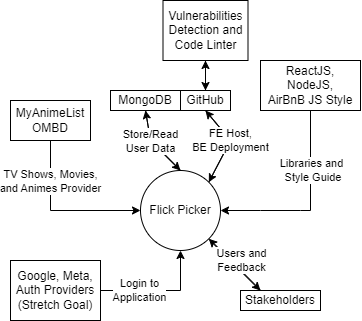
\includegraphics[scale=1]{contextDiagram.png}
\end{center}

\subsection{Work Partitioning}
\subsubsection*{Business Event List}
\begin{tabularx}{\textwidth}{|p{4cm}p{6cm}X|}
\toprule {\bf Event Name} & {\bf Input and Output} & {\bf Summary of BUC}\\
\hline
MyAnimeList/OMBD are polled & TV Show, Movie, and Anime Data (in) & Collect information about the shows to display to users \\
\hline
MongoDB data is updated & User data updated (out) & Any updates to user data are stored \\
\hline
MongoDB data is queried & User data retrieved (in) & Fetches everything needed for the user after login \\
\hline
Code is updated & GitHub redeploys new changes (in/out) & Updates the FE or BE deployment any time there is a merge to server \\
\hline
Deprecated library is used & Vulnerability detection blocks changes (in) & Deployment protection such that libraries are safe to use \\
\hline
Code does not match style & AirBnB style guide (in), Linter updates code (in/out) & Enforces the style guide on FE/BE development \\
\hline
External login is queried & External authentication validates user (in) & Allows users to log in with industry standard authentication providers \\
\hline
\end{tabularx}

\subsection{Specifying a Business Use Case (BUC)}
N/A as summary of BUCs are above.

\section{Business Data Model and Data Dictionary}
a

\subsection{Business Data Model}
a

\subsection{Data Dictionary}
a

\section{The Scope of the Product}
a

\subsection{Product Boundary}
a

\subsection{Product Use Case Table}
a

\subsection{Individual Product Use Cases}
a

\section{Functional Requirements}
a

\subsection{Functional Requirements}
a

\section{Non-Functional Requirements}
a

\subsection{Look and Feel Requirements}
a

\subsubsection{Appearance Requirements}
a

\subsubsection{Style Requirements}
a

\subsection{Usability and Humanity Requirements}
a

\subsubsection{Ease of Use Requirements}
a

\subsubsection{Personalization and Internationalization Requirements}
a

\subsubsection{Learning Requirements}
a

\subsubsection{Understandability and Politeness Requirements}
a

\subsubsection{Accessibility Requirements}
a

\subsubsection{Convenience Requirements}
a

\subsection{Performance Requirements}
a

\subsubsection{Speed and Latency Requirements}
a

\subsubsection{Safety-Critical Requirements}
a

\subsubsection{Precision or Accuracy Requirements}
a

\subsubsection{Reliability and Availability Requirements}
a

\subsubsection{Robustness or Fault-Tolerance Requirements}
a

\subsubsection{Capacity Requirements}
a

\subsubsection{Scalability or Extensibility Requirements}
a

\subsubsection{Longevity Requirements}
a

\subsection{Operational and Environmental Requirements}
a

\subsubsection{Expected Physical Environment}
a

\subsubsection{Wider Environment Requirements}
a

\subsubsection{Requirements for Interfacing with Adjacent Systems}
a

\subsubsection{Productization Requirements}
a

\subsubsection{Release Requirements}
a

\subsubsection{Backwards Compatibility Requirements}
a

\subsection{Maintainability and Support Requirements}
a

\subsubsection{Maintenance Requirements}
a

\subsubsection{Supportability Requirements}
a

\subsubsection{Adaptability Requirements}
a

\subsection{Security Requirements}
a

\subsubsection{Access Requirements}
a

\subsubsection{Integrity Requirements}
a
\subsubsection{Privacy Requirements}
a

\subsubsection{Audit Requirements}
a

\subsubsection{Immunity Requirements}
a

\subsection{Cultural Requirements}
a

\subsubsection{Cultural Requirements}
a

\subsection{Compliance Requirements}
a

\subsubsection{Legal Compliance Requirements}
a

\subsubsection{Standards Compliance Requirements}
a

\section{Project Issues}
a

\subsection{Open Issues}
a

\subsection{Off-the-Shelf Solutions}
a

\subsubsection{Ready-Made Products}
a

\subsubsection{Reusable Components}
a

\subsubsection{Products That Can Be Copied}
a

\subsection{New Problems}
a

\subsubsection{Effects on the Current Environment}
a

\subsubsection{Effects on the Installed Systems }
a

\subsubsection{Potential User Problems}
a

\subsubsection{Limitations in the Anticipated Implementation Environment That May Inhibit the New Product}
a

\subsubsection{Follow-Up Problems}
a

\subsection{Tasks}
a

\subsubsection{Project Planning}
a

\subsubsection{Planning of the Development Phases}
a

\subsection{Migration to the New Product}
a

\subsubsection{Requirements for Migration to the New Product}
a

\subsubsection{Data That Has to Be Modified or Translated for the New Product}
a

\subsection{Risks}
a

\subsection{Costs}
a

\subsection{User Documentation and Training}
a

\subsubsection{User Documentation Requirements}
a

\subsubsection{Training Requirements}
a

\subsection{Waiting Room}
a

\subsection{Ideas for Solutions}
a

\end{document}